\chapter{Conclusions and Future Work}\label{chap:chap4}

\section*{}

In this chapter is presented the conclusion of this report, including expected results and the work plan when working at this dissertation.

\section{Conclusion}
Since the beginning of \textit{Preparação da Dissertação} course, a lot has been learnt. From to develops scientific skills, such as, research from trustworthy resources, how to confirm that the resource and research is useful without wasting much time one it; to elaborate the related and formal reports and dissertations. To sum up, the first steps in the scientific field.

Many were the struggles and difficulties, but, in the end, this course is important to know where to start when working on the dissertations investigation/work.


\section{Expected Results}

What I expect from the work that will be developed during the dissertation period is the creation of an autotuner or concept proof that can achieve highest performance through available heterogeneous system components; consuming less energy compared to the old practices, like single but powerful CPUs or sequential code,  and saving programmers developing time when parallelizing code.
\section{Work Plan}
During the dissertation development, I plan the following tasks:
\begin{itemize}
    \item Learn how to use Kremlin;
    \item Apply Kremlin in an application;
    \item Result's analysis from Kremlin;
    \item Manually parallelize code on smart cities use case;
    \item Use Kremlin on smart cities use case;
    \item Compare results between manually and Kremlin;
    \item Manually parallelize code on biopharmaceutical use case;
    \item Use Kremlin on biopharmaceutical use case;
    \item Compare results between manually and Kremlin;
    \item Build autotuner /concept proof;
    \item Autotuner /concept proof result analysis;
    \item Write dissertation.
\end{itemize}

\begin{figure}[t]
  \begin{center}
    \leavevmode
    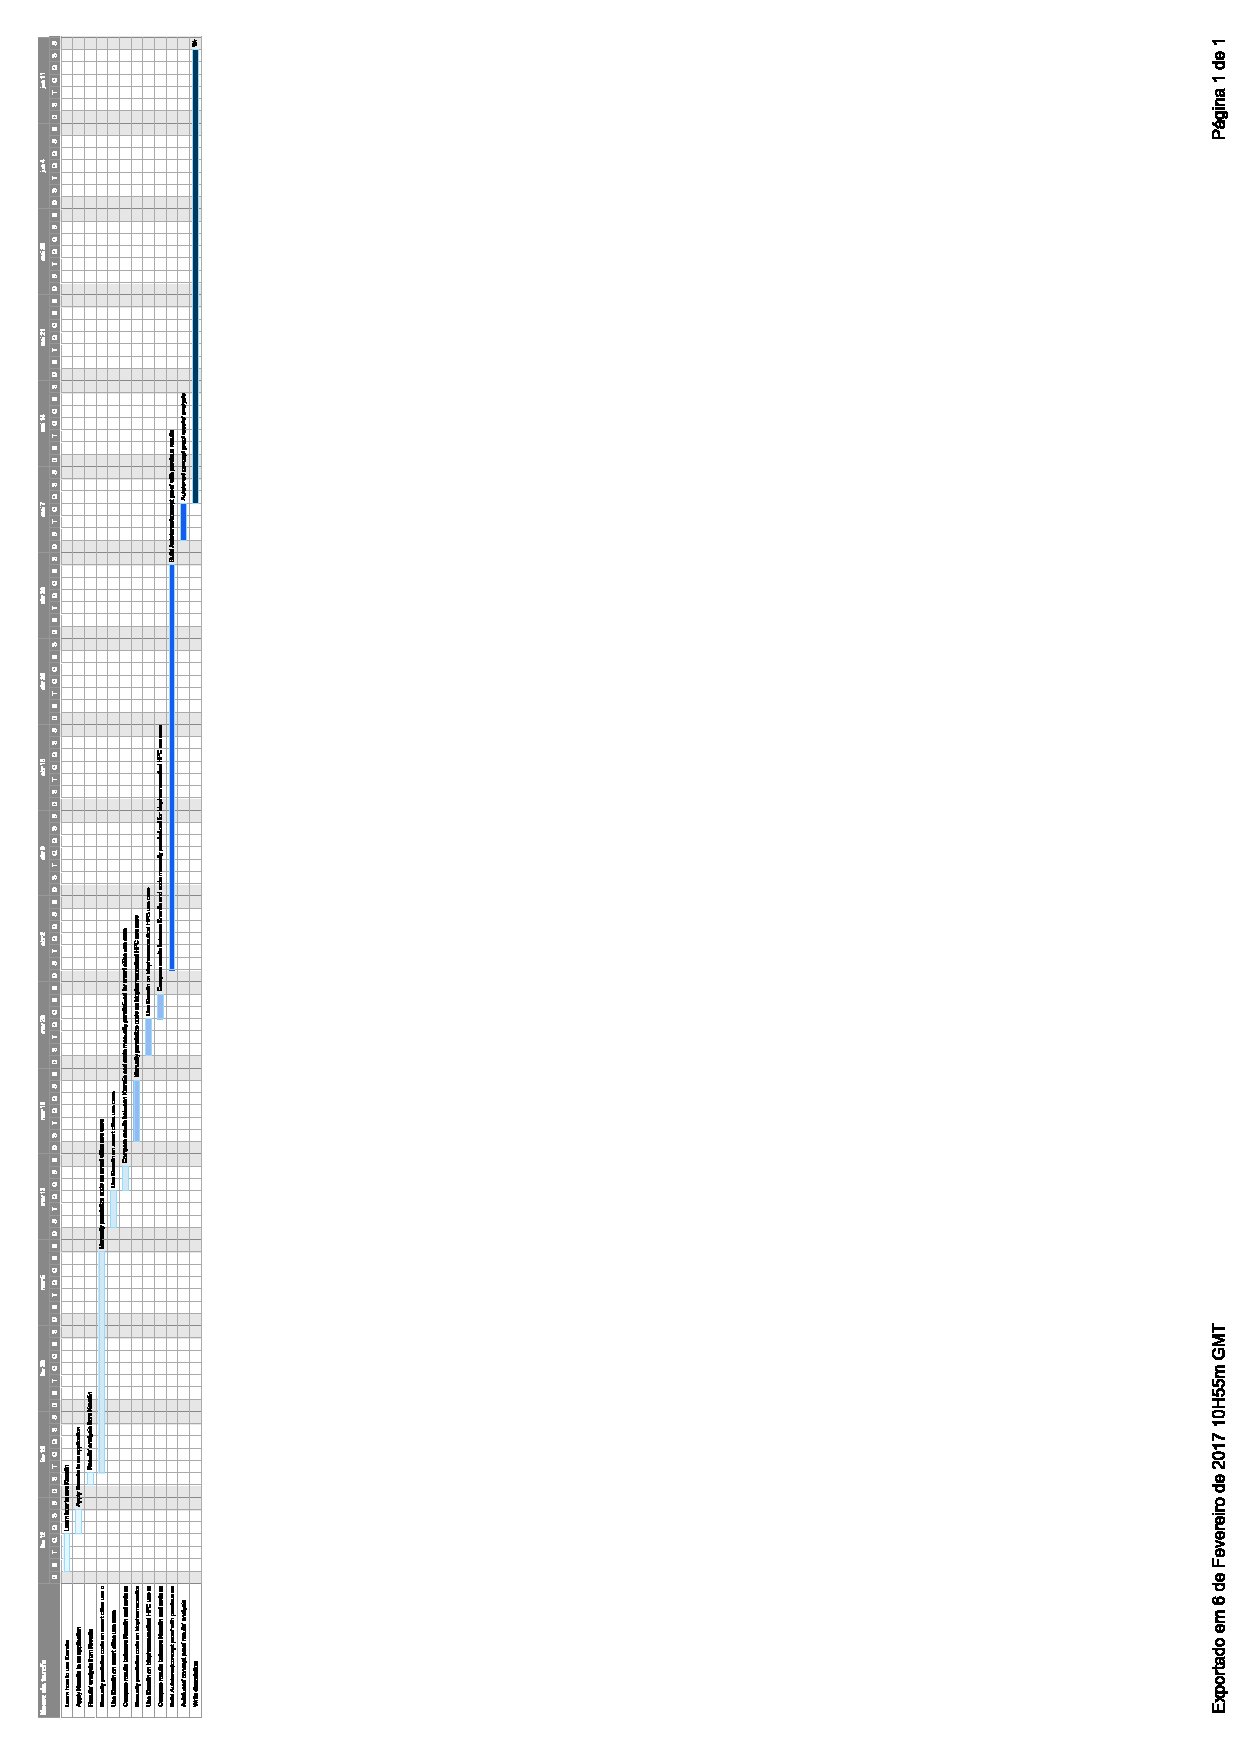
\includegraphics[width=1\textwidth]{workplan}
    \caption{Gantt's diagram for dissertation work plan}
    \label{fig:plan}
  \end{center}
\end{figure}
In figure \ref{fig:plan} is displayed the scheduling for the previous task list and their scheduled time, in the Gantt's diagram format. From previous task list, and the different choice of colors, this work plan can be divided in 5 phases: firstly, Kremlin know-how and knowledge; parallelization of the smart cities use case; parallelizations of the biopharmaceutical use case; build and validation of the autotuner; and finally, write dissertation. This work plan starts at February, thirteen, and is planned to finish at June sixteen.
